\documentclass[border=6pt]{standalone}
\usepackage{amsmath,amssymb}
\usepackage{tikz}
\usetikzlibrary{arrows.meta,calc,decorations.pathreplacing,patterns,shapes.geometric,positioning,shadings,plotmarks}

\begin{document}
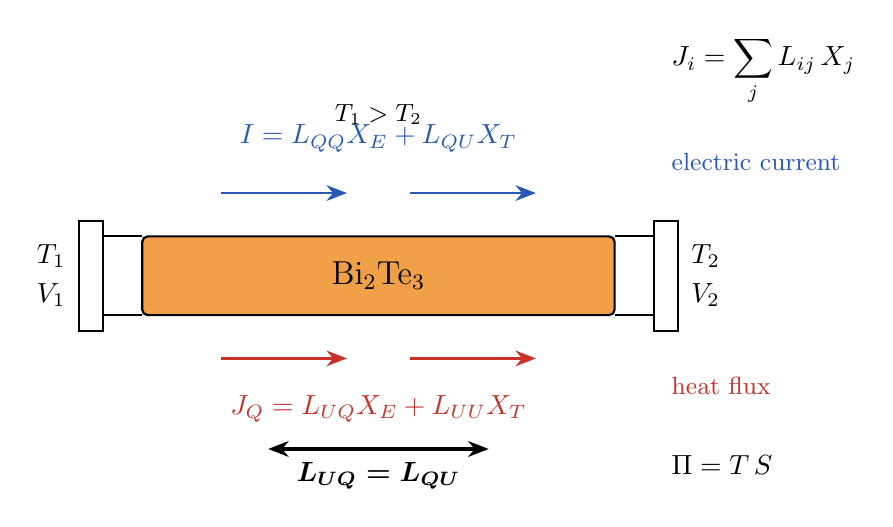
\begin{tikzpicture}[font=\rmfamily, >={Stealth[length=2.6mm,width=2mm]}]

% Equation top-right (general linear response)
\node[anchor=west] at (3.6, 2.6) {$J_i = \displaystyle\sum_j L_{ij}\,X_j$};

% Thermoelectric rod (orange)
\definecolor{rodorange}{RGB}{240,160,70}
\draw[fill=rodorange, draw=black, thick, rounded corners=2pt]
  (-3, -0.5) rectangle (3, 0.5);
\node at (0, 0) {\large Bi$_2$Te$_3$};

% Left contact (T1, V1)
\draw[thick] (-3, 0.5) -- (-3.5, 0.5);
\draw[thick] (-3, -0.5) -- (-3.5, -0.5);
\draw[thick] (-3.5, -0.7) rectangle (-3.8, 0.7);
\node[left] at (-3.85, 0.25) {$T_1$};
\node[left] at (-3.85, -0.25) {$V_1$};

% Right contact (T2, V2)
\draw[thick] (3, 0.5) -- (3.5, 0.5);
\draw[thick] (3, -0.5) -- (3.5, -0.5);
\draw[thick] (3.5, -0.7) rectangle (3.8, 0.7);
\node[right] at (3.85, 0.25) {$T_2$};
\node[right] at (3.85, -0.25) {$V_2$};

% Note T1 > T2
\node at (0, 2.05) {\small $T_1 > T_2$};

% Electric current I (blue) on top, left to right
\definecolor{currblue}{RGB}{40,90,180}
\draw[->, thick, currblue] (-2, 1.05) -- (-0.4, 1.05);
\draw[->, thick, currblue] (0.4, 1.05) -- (2, 1.05);
\node[currblue, anchor=south] at (0, 1.45) {$I = L_{QQ}X_E + L_{QU}X_T$};

% Heat flux JQ (red) bottom, left to right
\definecolor{heatred}{RGB}{200,50,40}
\draw[->, thick, heatred] (-2, -1.05) -- (-0.4, -1.05);
\draw[->, thick, heatred] (0.4, -1.05) -- (2, -1.05);
\node[heatred, anchor=north] at (0, -1.4) {$J_Q = L_{UQ}X_E + L_{UU}X_T$};

% Reciprocity double arrow below the heat label
\draw[<->, very thick] (-1.4, -2.2) -- (1.4, -2.2);
\node[anchor=north] at (0, -2.25) {$\boldsymbol{L_{UQ} = L_{QU}}$};

% Kelvin relation bottom-right
\node[anchor=west] at (3.6, -2.4) {$\Pi = T\,S$};

% Side labels for symbols
\node[anchor=west, currblue, font=\small] at (3.6, 1.45) {electric current};
\node[anchor=west, heatred, font=\small] at (3.6, -1.4) {heat flux};

\end{tikzpicture}
\end{document}
